\documentclass[10pt,letterpaper]{article}
\usepackage[margin=1in]{geometry}
\usepackage[T1]{fontenc}
\usepackage{lmodern,microtype,amsmath,amssymb,amsthm,booktabs,array,graphicx}
\microtypesetup{protrusion=false}
\usepackage{xurl}
\usepackage[hidelinks]{hyperref}
\hypersetup{pdftitle={Joint Deformation Costs: Technical Supplement},pdfauthor={Arnav Peram}}
\usepackage{enumitem,float}
\setlist{nosep,leftmargin=*}
\setlength{\parskip}{3pt}
\setlength{\parindent}{1em}
\renewenvironment{abstract}{\begin{center}\bfseries Abstract\end{center}\begin{quote}\normalsize}{\end{quote}}
\newtheorem{theorem}{Theorem}
\newtheorem{lemma}[theorem]{Lemma}
\newtheorem{proposition}[theorem]{Proposition}
\newcommand{\R}{\mathbb R}
\newcommand{\D}{\mathcal D}
\newcommand{\dist}{\operatorname{dist}}
\newcommand{\ind}{\mathbf 1}
\title{Technical Supplement: Joint Deformation Costs\newline for Continuous RNA-Ownership Sensitivity}
\author{Arnav Peram}\date{}
\begin{document}\maketitle
\noindent This supplement gives the exact constructions, source-clipping proof, native joint-cost and gene-count evidence, matched computational comparisons, and reproduction commands. All empirical analyses use the same selected development corridors and declared geometric settings.

\section{Exact critical-mesh reduction and the direct representation}
The canonical-realization lemma also supplies an exact finite-height route. The implementation is an exact reference construction using a shared integer-flow backend. Standard ordered-surface cuts supply the finite backend once sufficient candidates and costs have been derived.

\subsection{An ownership-independent common mesh}
Collect on each boundary every possible propagated lower/upper obligation term, fixed band/endpoint term, and source piece. Form a common mesh from their piece endpoints and every same-boundary isolated crossing. These are physical-input events, chosen before owners or molecular costs. Identical pieces do not create infinitely many crossings.

\begin{proposition}[Critical-mesh ownerwise equality]
For the absolute-displacement objective, restricting nodal heights to candidate-function values on this mesh, with the original constraints and trapezoidal nodal costs, preserves both feasibility and $D^\star(c)$ for every owner vector $c$.
\end{proposition}
\begin{proof}
Between mesh events every candidate piece is affine, candidate ordering is fixed, and all crossings with the source are included. Every canonical lower/upper envelope and clamp therefore selects affine pieces with constant-sign displacement. Its trapezoidal area is exact, and every nodal value is an available candidate. Thus a canonical minimizer for each feasible $c$ is retained at cost $D^\star(c)$.

Conversely, any feasible nodal candidate family interpolates to a continuous feasible family: the common mesh includes all source and obligation endpoints, and the slope, band, separation and interval-ownership constraints are linear between nodes. Absolute displacement on each affine interval is convex; its trapezoid upper-bounds its integral. That integral is at least $D^\star(c)$. The retained canonical realization gives the reverse inequality. Both directions prove the statement. Exactness of trapezoids is asserted for the canonical absolute displacement, not for every interpolant or arbitrary nonlinear loss powers.
\end{proof}

For candidates $v_0<\cdots<v_\ell$ at a surface/node pair, encode $H_k=\mathbf1[h\ge v_k]$, $k\ge1$, with $H_{k+1}\Rightarrow H_k$. The minimum candidate is unconditional. For $h_b\ge h_a+d$, every origin threshold implies the first destination threshold at least $v_k+d$; a missing destination forces the origin false. This includes the unconditional minimum constraint. Both directions enforce slopes and finite gap bounds. For an owner bit $b$, $b\Rightarrow h\ge L$ is a threshold implication, and $(b=0)\Rightarrow h\le U$ is its contrapositive $H_{\text{first value}>U}\Rightarrow b$. Apply obligations at every mesh node in their intervals. Trapezoidal absolute displacement and molecular terms are unary ordered-label costs, encoded by successive differences and constant shifts. Integer scaling gives an exact cut.

\subsection{Pruning, scope and graph size}
The reference gets the same ownership/pin closure as the direct compiler. Fixed-inactive cones are omitted. Fixed-active and geometric constraints give lower/upper envelopes which contain every feasible height. Crossings and candidates outside that interval are irrelevant to every canonical minimizer and are omitted. This is not a reward-dependent mesh. If all owners are forced, the reference reconstructs their canonical realization and skips height expansion; this also handles positive mandatory deformation.

Let $P$ count candidate affine pieces, $Q=O(P^2+P)$ the common event count, and $H=\sum_{b,j}(|V_{bj}|-1)$ the retained height bits. The reference graph has $Gm+H+2$ vertices and $O(H+NmQ+Gm)$ arcs, plus the retained redundant ownership-closure arcs. Candidate sorting and rational capacity scaling are polynomial. The direct graph instead retains molecular bits and merged integrated activation helpers. Neither formula implies a universal dominance or minimal graph-size theorem. The experiment below compares the explicit constructions, not every possible compressed surface graph.

At zero area penalty, a height-graph optimum need not be the least-area realization of its owners; area is unpenalized. It still attains the requested objective. Pinned ownerwise-area verification uses area coefficient one. The source-clipping shortcut and singleton upper bound require zero-deformation admissibility of every source ownership obligation, whereas the general representation permits source-inconsistent universal regions.

\subsection{Independent interval verification and exact mesh costs}
For baseline corridor \texttt{4037abe9fea38e}, a separate standard-library rational implementation reconstructs the 64 candidate vectors, 26 feasible costs, and the joint/additive optimizers without production kernels, realization, integration or cut routines. Primitive input ingestion remains shared. For each competing affine objective, strict positivity of its gap from the winner at both $67/100$ and $32/25$ proves uniqueness throughout the interval. The exact minimum endpoint gaps are positive for both objectives. The additive winner's regret under the joint-model objective is
\[
4-\lambda\frac{1060831597222835411423}{389056345355059200000},
\]
whose interval minimum is $154969482011724588577/303950269808640000000>0.5098514375$. The additive winner's unique-optimality interval is approximately $(0.6694696041,1.2829998335)$; endpoint ties are not claimed unique. The joint five-move optimizer extends to approximately $1.4260851948$.

\begin{center}
\begin{tabular}{lrr}\toprule
Objective & Gap at $\lambda=0.67$ & Gap at $\lambda=1.28$\\\midrule
Joint-model objective &0.721637496540&0.468202978465\\
Additive objective &0.000792262884&0.002338140238\\\bottomrule
\end{tabular}
\end{center}
These are the minimum gaps to \emph{any other feasible ownership vector} under the indicated objective, not the regret of the additive choice evaluated under the joint objective. All four are strictly positive by rational calculation. Exact fractions and closest competitors are in \texttt{results/endpoint\_gaps.json}; affine gaps give uniqueness throughout the closed interval.


\begin{figure}[ht]\centering
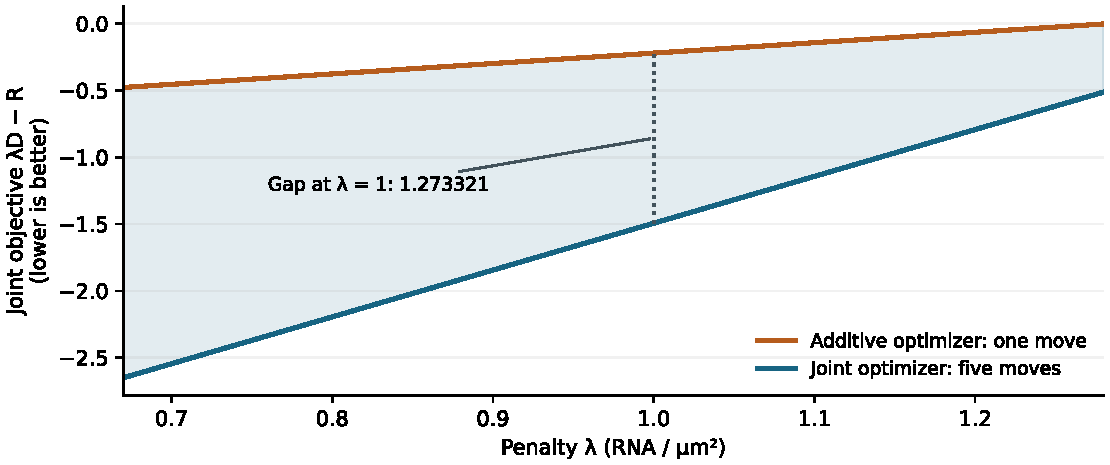
\includegraphics[width=.95\linewidth]{figures/native_penalty_interval.pdf}
\caption{Both selected owner vectors are evaluated with the same joint-model objective. The gap is positive throughout the verified closed interval; no geometry or observations change. The plotted coefficients are the separately enumerated exact costs.}\label{fig:interval}
\end{figure}

The audit's 52-node source/obligation mesh overestimates 25 of 26 canonical costs; its 888-node event mesh integrates every cost exactly. The reference optimizes its height-expanded graph. Safe pin-envelope pruning leaves 129 longitudinal nodes, 885 height bits and 25 owner bits, for 912 graph vertices and 3,675 arcs. The direct graph has 42 vertices and 308 arcs. Both optimize all three original penalties correctly and reproduce all 26 independently computed fixed-owner areas. The smaller reference mesh reflects safe preprocessing, not a change in the admissible model.

\section{Exact representation: input, assumptions and proof obligations}
The input contains $m$ ordered boundary functions on a compact interval $I$, rational piecewise-linear source curves, positive rational per-boundary slope limits, rational constant bands, fixed source endpoint values, and positive adjacent minimum gaps with optional finite maximum gaps. Exterior rails strictly enclose all bands. The source is geometrically admissible. Source admissibility under every universal RNA rectangle is a \emph{separate} assumption and is not required by the single-objective compiler. Fixed structural rectangles have pinned labels and universal semantics in every RNA mode. All structural rectangles count toward the input size.

For a group owner vector $c$, let $\mathcal F(c)$ be the entire continuous family realizing those owners and pins, and define
\[
 D^\star(c)=\min_{f\in\mathcal F(c)}\sum_a\int_I|f_a-f_a^0|\,dt,
 \qquad \min\varnothing=+\infty.
\]
The representation has molecular threshold vertices $b_{ga}=\mathbf1[c_g\le a]$, helper vertices $y$, rational finite capacities, and formal hard arcs. Feasibility means there exists a helper assignment cutting no hard arc. For every feasible $c$,
\begin{equation}
 \min_y \operatorname{Cut}_{G_D}(b(c),y)+\kappa=D^\star(c).\label{eq:ownerwise}
\end{equation}
The constant $\kappa$ is known and independent of $c$; it is zero before mandatory analytic terms are extracted. An integer implementation divides its finite cut value by a recorded common denominator before adding $\kappa$. Hard capacities are selected above the sum of all finite capacities for the optimized objective. The graph either proves infeasibility or produces an owner vector and rational attaining curves.

\subsection{Why nodal feasibility is a different result}
A finite mesh containing endpoints and every obligation-interval endpoint exactly represents \emph{feasibility} with real-valued nodal heights and discrete owners. Sampling maps a continuous feasible boundary to feasible nodes. Linear interpolation maps feasible nodes back: bands, adjacent gaps, slope inequalities, and interval ownership inequalities are linear on each subinterval. Including source knots is harmless. Thus the existence of finite nodal feasibility, or avoiding an externally supplied candidate-height menu, is not a distinct novelty claim here. The stronger assertion in~\eqref{eq:ownerwise} eliminates those real coordinates while preserving their exact integrated minimum for \emph{every} owner vector. A trapezoidal objective on that mesh need not have this property.

\subsection{Both directions of the geometric constraints}
Let $\Delta_{ab}$ be the maximum path weight of the directed gap constraints, including reverse edges of weight minus each finite maximum gap. Let
\[
 K_{ab}(r)=\max_c\{\Delta_{ac}+\Delta_{cb}-s_c r\}.
\]
A source-feasible system has no positive gap cycle. These kernels are the exact closure under finite sequences of longitudinal Lipschitz and same-coordinate difference constraints. For a direct edge $a\to b$ of weight $d$, path composition gives
\[
 K_{ob}(r)\ge K_{oa}(r)+d,\qquad
 K_{ao}(r)\ge d+K_{bo}(r).
\]
Therefore propagated lower envelopes satisfy $L_b\ge L_a+d$, and propagated upper envelopes satisfy $U_a\le U_b-d$. Applying these facts also to each reverse maximum-gap edge establishes \emph{both} gap inequalities. Terms whose longitudinal rate exceeds the destination rate are dominated by the direct destination term; hence the output envelopes meet the correct slopes. Propagated bands and fixed endpoints are included as constraints, not presumed after construction.

For a lower interval $(a,I_i,\ell_i)$ and an upper interval $(b,I_j,u_j)$, the necessary and sufficient conflict test is
\[
 \ell_i+K_{ab}(\dist(I_i,I_j))>u_j.
\]
Unary tests apply the same path inequalities to bands and fixed endpoints. A lower obligation is impossible if a propagated value exceeds a destination upper band or endpoint; upper obligations are symmetric. Fixed structural owners impose all their nested bits, so their interval inequalities participate in the same tests. A positive conflict gives the appropriate owner-bit implication. The pairwise/unary conditions imply $L_b\le U_b$ everywhere through kernel composition and the triangle inequality.

The family of difference-potential constraints is closed under componentwise minimum and maximum. Since $L,U,f^0$ obey its geometry,
\[
 f_b^*(t)=\min\{U_b(t),\max\{L_b(t),f_b^0(t)\}\}
\]
is jointly feasible. It is the nearest permitted coordinate to $f_b^0(t)$ at every $(b,t)$, so its displacement magnitude is pointwise no greater than that of any realizing family. This is the simultaneous-attainment step. Lattice closure itself and Lipschitz envelopes are established tools.

\subsection{Analytic integrated cost and repeated activations}
On each destination boundary and polarity, every molecular obligation contributes a nonnegative source-relative excursion function. Source owners need not satisfy a whole uncertain rectangle, so non-flip obligations cannot be discarded. Fixed structural terms remain included. A feasible ownership vector's upward and downward excursions do not overlap positively on the same boundary.

Split the domain at all source knots, obligation plateau endpoints, zeros, and positive intersections. On a slab, ordered affine heights $h_1\ge\cdots\ge h_k>0$, with $h_{k+1}=0$, give
\[
 \max_{j\text{ active}}h_j
 =\sum_{j=1}^k(h_j-h_{j+1})\,
       \mathbf1[\text{an active variable belongs to }S_j].
\]
Integrate each nonnegative affine difference exactly. If several cones have the same activation bit, the prefix set contains that bit once. Both activation polarities use their corresponding standard cut gadgets. Fixed-positive terms contribute a constant or a forced helper, not an omitted cost. These identities hold for every hard-feasible owner assignment, which proves~\eqref{eq:ownerwise}, not merely equality of one optimized answer.

\subsection{Encoding and losses}
$N$ counts all merged RNA and structural obligation rectangles; $J$ counts source knots. The full arrangement still has $O(M_b^2+M_bJ_b+J_b+1)$ slabs on boundary $b$, and the implementation may scan $M_b$ raw layers on each. The aggregated graph is smaller than that raw work bound: the prefix-family proposition below gives $O(M_b^2+M_b)$ helpers. Rational coordinates, integration, constant shifts and denominator scaling retain polynomial bit complexity. The graph-size improvement does not remove source knots from integration work or capacity encoding, nor prove optimal construction time.

Pointwise minimum displacement also minimizes any separable loss $\sum_b\int\psi_b(t,|f_b-f_b^0|)dt$ that is nondecreasing in its nonnegative second argument, provided the losses are measurable and their compositions with admissible displacements are integrable. This is an immediate consequence, not an additional general optimization paradigm. Arbitrary monotone functions do not automatically have a finite exact arithmetic representation. Fixed-degree polynomial powers do: on each ordered slab the transformed layer differences are nonnegative fixed-degree polynomials with exact rational integrals. Their degree must enter the resource bound.


\section{Complete source-clipping argument and implementation guard}
Fix the corridor, included groups, source vector $b^0$, source geometry $f^0$, fixed regions, and all physical constraints. Let $\mathcal B$ be the base finite implication system. The shortcut assumes that $f^0$ realizes \emph{every} source-owner obligation at zero cost, not merely that $f^0$ is geometrically admissible. The constructor directly checks this assumption. It distinguishes an inconsistent base model from a nonadmissible source; neither is reported as meaningful RNA preservation.

For any owner pins, propagate all required true bits forward and required false bits backward. If these sets intersect, a path from a required true bit to a required false bit certifies infeasibility. Otherwise let $T,F$ be the closures and put $\widehat b=1$ on $T$, zero on $F$, and equal to $b^0$ elsewhere. For an implication $u\Rightarrow v$, a true $u\in T$ forces $v\in T$; a false $v\in F$ forces $u\in F$. When both remain free the source satisfies the implication. The mixed cases cannot introduce a violation. Nesting and structural pins are included among these implications and fixes. Thus $\widehat b$ is feasible.

Every obligation active at the source contributes zero positive source-relative excursion after propagation, since the source itself satisfies all geometry. A costly obligation activated by $\widehat b$ comes from a bit forced away from the source. Every feasible completion activates that same obligation. The upward/downward excursion maxima for $\widehat b$ are therefore pointwise no larger than those for any completion. The canonical clamp realizes these maxima simultaneously. Integration proves exact minimum deformation, not merely a lower bound.

After preparing the implication graph, a query traverses $O(V+E)$ graph structure. Envelope construction, integration, and original-coordinate checking have separate polynomial costs. The implementation preserves full constraints on unpinned RNA, allowing collateral ownership changes only when forced. It is not equivalent to constructing one isolated scalar tent and ignoring other obligations.

The audit enumerates 5,589 vectors from 140 source-feasible small models and asks 2,867 single/multiple-pin questions: 1,767 are feasible and 1,100 infeasible. Direct fixed-owner enumeration agrees in every case. An explicit universal rectangle straddling the source tests rejection of the stronger premise. The 1,132 native alternative-owner questions all match archived costs and feasibility. The 732 pair queries also match this shortcut. The independent closure checker uses set propagation and direct geometry checks; its base implication system is shared, so it is not an independent theorem proof.

\section{Joint cost, additive overestimation, and identifiability}
For each destination $o$, define $d_g(o)=\min_{c:c_g=o}D^\star(c)$; set $d_g(c_g^0)=0$. If $c$ is jointly feasible, each singleton closure is compatible with it. Every newly activated costly obligation in $c$ is activated directly by the pin for its own group, and any further obligation forced by such a pin must also be active in $c$. Therefore the joint upward and downward excursion maxima are the maxima over the singleton completions. Their integrals are bounded by the sum of the corresponding singleton integrals:
\[
D^\star(c)\le\sum_g d_g(c_g).
\]
The inequality uses zero-cost source admissibility and the positive maximum-envelope cost. It is not asserted for a source already violating its RNA-region obligations, an arbitrary objective, or an infeasible owner vector.

\paragraph{Same singletons and feasible set, different joint optimum.}
Take flat source zero on $[0,3]$, slope one, band $[-1/2,1/2]$, clearance $1/20$. Two right-owned RNA have transverse coordinate $1/5$. Let their longitudinal coordinates be $(1,5/4)$ in system A and $(1,2)$ in system B. Every owner vector is feasible in both systems, and both singleton costs are $1/16$. Their joint costs are $7/64$ and $1/8$, respectively. At reward $3/50$ per changed RNA and area multiplier one, both systems have singleton objective $1/400$. System A has joint objective $-17/1600$ and changes both; system B has joint objective $1/200$ and preserves both. Thus exact feasible owners and exact singleton thresholds do not determine the optional optimum. The construction is directly checked against all four fixed-owner patterns and the integrated cut. It is an information-loss example, not a new general impossibility theorem about optimization.

\paragraph{Surrogate definition and favorable tie handling.}
Use $E_A(c)=\lambda\sum_gd_g(c_g)-R(c)$ over the identical exact feasible set. The source minimizes neither objective by definition; it is merely one feasible candidate. Costs for infeasible singleton labels can be placeholders only because exact hard restrictions exclude them. The audit asserts that no such label is selected.

Let $L$ be a common denominator making every surrogate unary contribution integral. Choose integer $M>\lambda B+W$, with $B=|I|\sum_a(\overline b_a-\underline b_a)$ and total charged weight $W$. A distinct surrogate primary value differs by at least $1/L$, while the range of $E$ is at most $\lambda B+W$. Optimizing $ML E_A+E$ therefore first minimizes $E_A$, then minimizes $E$ over its minimizers. The graph represents this objective by keeping the true area coefficient $\lambda$ and adding the scaled surrogate unary costs. The recorded lexicographic certificate has a scaled combined objective; it is not confused with the separately recomputed joint-model objective. Every primary optimum is cross-checked.

The comparator intentionally gives the additive method access to the true joint representation \emph{only for favorable evaluation of its ties}. Any positive regret survives every possible primary-optimal tie choice, including a deployable simpler tie rule. It is not a fair claim that this diagnostic is cheaper than the true method. On 100 independent small test panels, exhaustive enumeration of 2,500 vectors checks all 300 primary/secondary choices and 559 feasible-vector additive inequalities with no discrepancy.

\section{Full native optional-decision results}
\paragraph{Corridor selection.}
The source masks are scanned along both coordinate orientations. A candidate must retain one ordered sequence of nonzero cell labels over the entire window; outer rails, source ownership, clearance and every intersecting nuclear region must be compatible. RNA eligibility is 3--24 sites. The original 24-row three-cell screen yielded zero eligible windows; the exploratory amendment admitted fixed nuclear regions, shorter windows and two-cell cases. Eligible charts are chosen by deterministic hash order, nonoverlap within each ROI/setting, and a cap of 12 per ROI/setting. The final set has eight three-cell and 34 two-cell corridors. These development choices and overlapping windows prevent interpreting coverage as a tissue-wide sampling estimate.

The fixed protocol uses 42 original corridors, their baseline and largest existing geometric settings, and penalties $1/4,1,4$. No parameter is tuned after inspecting the new optional results. All 252 questions are retained; illustrative cases are selected afterward. Both models use the same exact feasibility, nuclei, observations and clearance.

\begin{center}
\begin{tabular}{lrr}\toprule
Quantity & Baseline & Largest family\\\midrule
Queries &126&126\\
Strict joint-model objective regret, even after best tie &1&16\\
Corridors with such a query &1&12\\
Exact optimum with cost below singleton sum &18&48\\
Surrogate preserves all while exact changes &0&0\\\bottomrule
\end{tabular}
\end{center}
There are 12 distinct affected corridors overall. The 235 zero-regret questions remain included. All 17 positive-regret questions also change counts, not merely labels. Different counts need not imply a biological classification change.

\paragraph{Baseline example with complete owner enumeration.}
Corridor \texttt{4037abe9fea38e} has source cells 153124 (left) and 153133 (right). At $\lambda=1$, the exact solution changes the five RNAs below right-to-left. The surrogate selects LTBP2 left-to-right instead. The original source and nuclear constraints are unchanged.
\begin{center}
\begin{tabular}{lrl}\toprule
RNA gene & Global transcript identifier & Selected move\\\midrule
PECAM1 &281689725216814&right $\to$ left, joint\\
TMEM100 &281689725244142&right $\to$ left, joint\\
MYC &281689725293591&right $\to$ left, joint\\
C7 &281689725391569&right $\to$ left, joint\\
PMP22 &281689725449663&right $\to$ left, joint\\
LTBP2 &281689725226245&left $\to$ right, additive\\\bottomrule
\end{tabular}
\end{center}
The joint area is exactly
\[
\frac{143227474810907125420487}{40850916262281216000000},
\]
and the additive optimizer's true area is
\[
\frac{8257302153140406437}{10594117287936000000}.
\]
The joint-model objective regret is
$495393784197401388577/389056345355059200000$.
The five joint moves have summed singleton area approximately $8.696707$, but joint area approximately $3.506102$. A separate fixed-owner enumeration checks all 64 candidate vectors, 26 feasible, and independently reconstructs the primary and favorable-secondary optima at every tested penalty. This proves the case's reported decisions without requiring confidence in the min-cut backend. It shares the fixed-owner continuum formulation.

\section{Joint feasibility and the native minimum-thickness obstruction}
The pair census keeps the source model fixed. Every pair of individually movable records is considered, with all feasible alternative-owner combinations. These are post-hoc dependent questions on the development corridors.
\begin{center}
\begin{tabular}{lrr}\toprule
Quantity & Baseline & Largest family\\\midrule
Pair questions &80&652\\
Jointly infeasible &22&85\\
Jointly feasible &58&567\\
Joint cost below sum of singleton thresholds &23&144\\
Joint cost equal to sum &35&423\\
Finite cost equals two-target scalar bound &56/58&567/567\\
Impossible pair explained by own-boundary slope &22/22&84/85\\\bottomrule
\end{tabular}
\end{center}
Separate implementations agree on these values. The successful scalar comparisons are retained: joint cost savings alone do not demonstrate a need for the complete compiler in a \emph{pinned} query. Optional selection and pinned reconstruction are different tasks.

In corridor \texttt{c8f8188430d092}, both target RNAs start in middle cell 153955. MDM2 is transcript 281689725326771 (group 14). TFPI is transcript 281689725446833 (group 19). MDM2 to right cell 153965 costs $0.9068512714$, and TFPI to left cell 153959 costs $1.1046851294$, in summed interface $\mu$m$^2$. Both targets are impossible together with the original minimum gap, also after dropping only the maximum gap. Replacing only the minimum gap $\frac{2097152}{1644825}$ by the band-implied $\frac{904654}{1644825}$ makes the joint change feasible at cost $2.0115364008$.

The TFPI lower requirement transmitted to the right boundary by slope 2 and the original minimum gap exceeds the MDM2 upper requirement by exactly $187707749/4210752000\,\mu$m. Figure~\ref{fig:conflict} plots these requirements. The horizontal dashed height is the MDM2 restriction \emph{at its coordinate}, not a new constant upper bound across the interval. This is a one-inequality proof of a coupled infeasibility, not evidence that optimization is necessary to discover every obstruction.
\begin{figure}[h]\centering
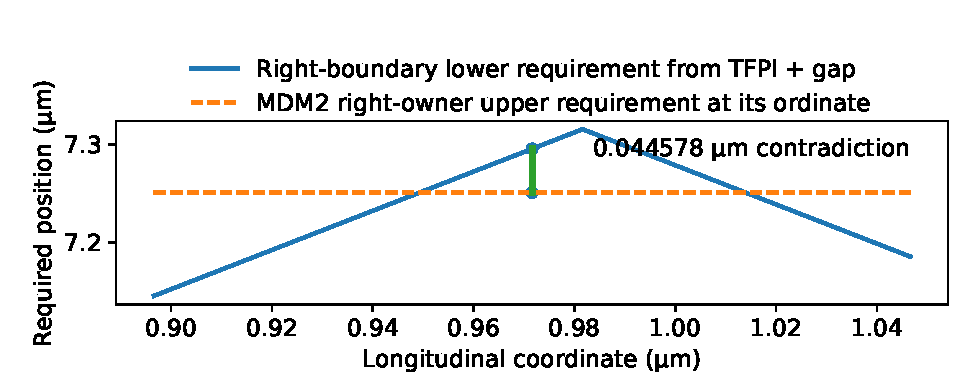
\includegraphics[width=.95\linewidth]{figures/native_thickness_obstruction.pdf}
\caption{The two requested owners cannot coexist: at the MDM2 ordinate the propagated lower requirement is above its allowed upper value. Individual counterexamples are valid; their simultaneous use is not. The relaxed joint witness is never labeled feasible under the original model.}\label{fig:conflict}
\end{figure}

\section{Corridor conditioning and interpretation of the parameter range}
Report $d_{g\to j\mid\mathcal C,\theta}$ together with the corridor, source-cell and destination-cell identities. The continuous parameter box varies only endpoints, slope and bands within that fixed construction. Extending a smaller-family boundary by source-constant pieces into the largest domain adds no cost or observation, and relaxed bands/slopes preserve feasibility. Thus the infimum within that fixed corridor equals the largest-family threshold. Changing the corridor or neighbor set is outside the quantified box.

For 54 repeated global transcript/source/destination combinations, the exact overlap audit gives:
\begin{center}
\begin{tabular}{lrr}\toprule
Outcome across corridors & Baseline & Largest family\\\midrule
Finite in one, impossible in another &6&3\\
Unequal finite thresholds &0&4\\\bottomrule
\end{tabular}
\end{center}
For example, MYC transcript 281689725293591 can move from 153133 to 153124 in corridor \texttt{4037abe9fea38e}, at largest-family cost about $1.072506\,\mu$m$^2$, but is band-excluded in \texttt{a0987140ecb03c}. The latter includes a different neighbor configuration and separately fitted bands. These are distinct conditional model outputs, not conflicting measurements of a single intrinsic RNA threshold. No averaging or automatic global stitching is performed.

The 928 per-record per-setting minimum thresholds include 219 finite values and 709 infinite values. All 171 finite largest-family values attain own-boundary scalar bounds; 47/48 finite baseline values do. Nonincrease under the nested relaxation is proved, not itself a biological finding. Native finite ratios can also reflect elementary tent scaling such as $(h+\rho)^2/s$ for a flat isolated target. Magnitudes and changed decisions must therefore retain their model-conditioning interpretation.

\section{Matched threshold workload and graph reuse}
Every run evaluates all 1,132 destination-specific queries for the same 84 corridor/setting models. Data parsing, imports and creation of the immutable input objects are outside the clock. Included work is method preparation, query closure or compilation, graph construction, flow where used, rational reconstruction, graph or closure checking, and continuous-boundary verification. No RNA subset or difficult case is dropped. Three fresh processes per method use a shuffled method/replicate schedule, requested single-thread BLAS and solver settings, and no exclusive CPU affinity.

\begin{center}
\begin{tabular}{lrrr}\toprule
Method & Median (s) & Range (s) & Peak process RSS (MiB)\\\midrule
Per-pin recompilation &19.263&19.032--19.506&175.79--175.80\\
Compile once + late pins &5.618&5.404--6.199&175.80\\
Pin closure + reconstruction &4.611&4.333--4.707&174.92--174.94\\\bottomrule
\end{tabular}
\end{center}
RSS includes imports and shared dependencies. It does not establish an isolated memory improvement. The reference code prepares a separate immutable graph for each corridor/setting, reuses its capacities for late positive pins, and solves each flow anew. No dynamic-residual warm start is claimed. In both cut modes every flow/cut and boundary is checked. The shortcut substitutes a checked closure proof and reconstructed boundary, not a flow proof for a graph it never builds.

\begin{center}
\begin{tabular}{lrrrr}\toprule
Per-model query prefix &1&4&16&All\\\midrule
Per-pin recompilation, aggregate seconds &0.877&3.601&12.550&19.263\\
Compile-once reuse &1.440&2.216&4.230&5.618\\
Pin-closure shortcut &0.788&1.427&3.358&4.611\\\bottomrule
\end{tabular}
\end{center}
Prefixes are derived from the same full executions and include model setup; models with fewer queries contribute all available queries. They are not a separate randomized crossover study. Reuse amortizes its preparation, whereas the shortcut avoids area layers. Reconstructed areas agree exactly across all nine runs. The main remaining shortcut cost is reconstruction (median about 3.404 s); graph traversal itself takes about 0.016 s. Retained reusable graphs contain 6--76 vertices and at most 698 arcs.

A separate active-coupling construction with five cells and 96 RNA groups completes in approximately 10.41 seconds, almost all in compilation; its 384-group case reaches the 40-second limit during compilation. All eight tested settings, including that failure, remain in the historical companion. This excludes a broad scalability claim.

The inherited constructed family has compilation times 0.152, 2.102 and 32.078 s for 24,96,384 groups. This near-quadratic observed growth coexists with roughly linear output-size growth; pairwise processing remains an optimization opportunity. No locality-speed claim is added here, and no timeout is replaced by a fictitious solve time. The old caching-controlled 84-objective result is retained only as the compiler ablation, not as the timing for this 1,132-query application.

\begin{figure}[ht]\centering
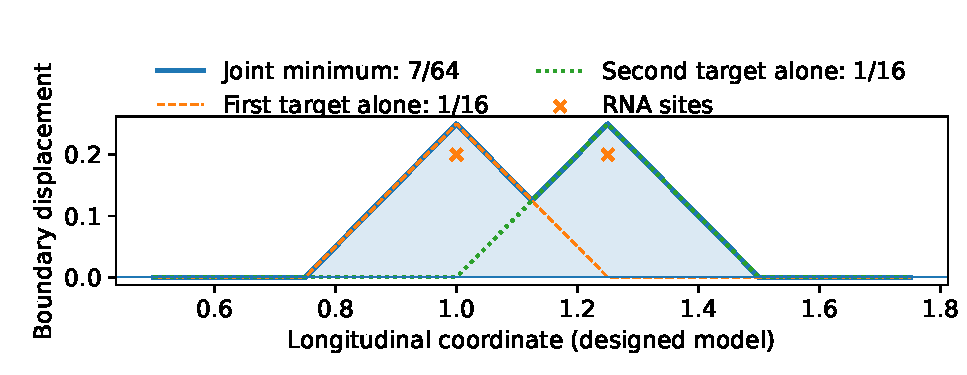
\includegraphics[width=.92\linewidth]{figures/shared_deformation.pdf}
\caption{Constructed two-site shared deformation. Individual areas are $1/16$ each; simultaneous area is $7/64$, below their sum. This is a model illustration, not native tissue.}\label{fig:shared_supp}
\end{figure}

\section{Prefix-family aggregation: a tighter graph-size bound}
For one output boundary and polarity, let $M$ count propagated untruncated terms
\[
 g_i(t)=\alpha_i-s_i\dist(t,I_i).
\]
The positive excursion is $[g_i(t)-r(t)]_+$, with a common piecewise-affine reference $r$; using $r=-f^0$ covers the other polarity. The same argument applies after pin substitution replaces $r$ by a mandatory envelope.

\begin{proposition}[Quadratic prefix-family bound]
After merging identical activation sets, $O(M^2+M)$ helper vertices and helper arcs suffice for this boundary/polarity, independently of the number of reference knots. Across all boundaries, the main-text bounds in equation (15) follow, with auxiliary contribution $O(N^2m^5)$ when $M_b=O(Nm^2)$.
\end{proposition}
\begin{proof}
Each $g_i$ has at most three affine pieces. For a pair, their combined breakpoints split the domain into at most five intervals; on each their difference is affine. Hence their ordering changes only constantly many times, including transitions into and out of coincidence intervals. Choose a fixed index tie rule on every open interval. Consecutive orderings differ by adjacent swaps, with the total number of swaps bounded by the total pair-order changes, $O(M^2)$. A block of simultaneous crossings can be expanded into such swaps for counting; hypothetical intermediate prefixes only enlarge the family and preserve the upper bound.

One ordering has at most $M$ nonempty cone-index prefixes. An adjacent swap changes just the prefix ending between the swapped positions. Thus the union of all prefixes has size $O(M^2+M)$. The common reference changes which terms are positive but not their relative order: the positive terms are an initial segment of the same ordering. Every nonzero layer therefore uses one of the counted prefixes. Mapping cone indices to their activation labels cannot increase the number of distinct sets, even when several cones carry the same bit.

For each new activation set $S$, choose an occurrence of its prefix and the last newly appearing label $v$ there. The preceding distinct-label prefix is $P=S\setminus\{v\}$. Retain $P$ even if its aggregate weight is zero, and connect its helper and $v$ to the helper for $S$ (reverse the implications for complement polarity). Cardinalities strictly decrease down predecessor links, so the construction is acyclic and uses constant arcs per set. Every required predecessor is another prefix in the same counted family; no additional asymptotic factor appears. Sum exact weights from every slab and every repeated occurrence.

Summing over both polarities and all destinations gives $O(\sum_b(M_b^2+M_b))$ helpers. Owner bits add $O(Gm)$ vertices; nesting, unary pins and ownership implications add $O(Gm+N^2m^2)$ arcs. This proves the stated graph-size bound.
\end{proof}

This is an existence/aggregation bound, not a kinetic construction-time theorem. Source knots and zeros may generate many integration slabs; the present implementation scans layers before merging. Source geometry also changes integrated rational weights and their bit lengths. No lower bound for all compressed height encodings is asserted. New rational checks cover 168 polarity-arrangements, 1,260 activation assignments and 484 predecessor-helper identities, including simultaneous events, coincident functions, repeated labels and 41-knot oscillatory references. Test truth integrates selected maxima separately from the production layer routine.

\section{Hard-implication SCC contraction}
For any hard-feasible cut, vertices in one strongly connected component of the hard-arc graph have the same Boolean label. Contract them and sum parallel capacities; self-arcs vanish. Feasible original cuts and quotient cuts then correspond by lifting, and all finite costs agree. This holds for each fixed owner vector, hence preserves its minimum auxiliary cost. The contraction depends only on hard constraints and is reused across molecular objectives. New pins require a new hard-constraint partition; it cannot be reused after silently changing the feasible family. If source and sink belong to one hard SCC, retain an infeasibility certificate rather than merge them into a valid terminal.

This is standard graph contraction. Both representations receive the identical implementation. Tests compare all 1,523 hard-feasible cuts across 200 small graphs and 72 optional objective questions on 24 physical models. Lifted cuts are checked against original cut capacities; continuous boundaries are checked at original coordinates.

\subsection{Current SCC same-workload measurement}\label{sec:current_scc}
All 84 models, 252 objectives and physical assumptions are unchanged. There are three fresh sequential processes for each representation/contraction condition, twelve completed runs in total. Preparation includes the SCC partition, and each query includes quotient construction, integer flow, checking, lifting, reconstruction and geometric checking. The area/molecular graph is rebuilt with new capacities; no residual-flow warm start is claimed. The allowance is 30 seconds per model; none reaches it. Only completed fresh-process runs enter the table; execution provenance is retained in the artifact.

\begin{center}
\begin{tabular}{lrrrr}\toprule
Workflow & Compile (s) & SCC prep. (s) & Queries/checks (s) & Median total (s)\\\midrule
Direct &1.216202&0.000042&3.027794&4.265857\\
Height &13.866863&0.000047&11.977717&25.927651\\
Direct + SCC &1.321135&0.016847&3.121761&4.530190\\
Height + SCC &13.978759&0.338018&4.931485&19.539520\\\bottomrule
\end{tabular}
\end{center}
Tiny non-SCC prep values are timer overhead. Every stage entry is a median across three processes; separate medians do not add exactly. After SCC, the height/direct ratios are approximately 10.58 for compilation, 1.58 for queries/checks, and 4.31 for the complete workload. The total ratio is not a per-query acceleration factor. After SCC contraction, the optional subset has 48 models/144 queries, aggregate medians 3.417287 seconds (direct) and 19.041921 (height), and median per-model height/direct ratio 3.884287. All 48 favor direct. The 36 fixed models/108 queries favor height in every case: aggregate medians 1.076773 and 0.494329 seconds, median per-model ratio 0.444829. The caching asymmetry is retained and stated, not attributed to representation theory. Direct SCC overhead slightly increases its total relative to the already small raw graphs.

All 3,024 query objectives agree with the exact archived values. Graph sums after SCC are 1,431 vertices/7,855 arcs (direct) and 6,473/27,010 (height), compared with 1,806/13,212 and 37,052/149,120 before. The summed-vertex ratio after contraction is approximately 4.52, not a mean per-instance compression ratio. In the showcase the graphs contract to 37 vertices/210 arcs and 187/803, respectively. No asymptotic or state-of-the-art dominance is inferred.


\begin{center}
\begin{tabular}{lrr}\toprule
Current workflow & Minimum total (s) & Maximum total (s)\\\midrule
Direct&4.158397&4.321719\\
Height&25.532431&27.739519\\
Direct + SCC&4.300802&4.586318\\
Height + SCC&17.816716&19.625011\\
\bottomrule
\end{tabular}
\end{center}
These are minimum and maximum observed process times, rather than confidence intervals.

\subsection{Actual exact-benchmark environment}\label{sec:current_environment}
The current twelve-process SCC census records an AMD EPYC 9V74 80-Core Processor, Linux 6.18.55 x86\_64 with glibc 2.41, and CPython 3.13.5 (GCC 14.2.0), directly in \texttt{results/environment.json}. The visible topology reports one socket, five cores per socket, and one thread per core; the processor model name is not a claim that 80 cores were allocated. Recorded imports are NumPy 2.3.5, SciPy 1.17.0, NetworkX 3.6.1, Matplotlib 3.10.8 and PyMuPDF 1.26.7. The experiment requests one thread via \texttt{OMP\_NUM\_THREADS}, \texttt{OPENBLAS\_NUM\_THREADS} and \texttt{MKL\_NUM\_THREADS}, with \texttt{PYTHONHASHSEED=0}, and reserves no exclusive core. Exact flow uses Python integers, not BLAS. Benchmark RSS includes common imports; the portable standard-library replay has a different import footprint and is not substituted into the timing or memory tables.

\section{Gene-count readout audit}
The readout audit uses all original 42 corridors, both geometric settings and all three penalties. Every original question and every gene is retained. Detection uses the elementary count threshold $n>0$. This is a post-hoc interpretation of development-data queries, with each corridor considered separately.

\paragraph{Source reconstruction.}
\texttt{experiments/build\_readout\_inputs.py} reads both retained Parquet crops with PyArrow and checks all 7,370 records against cell-mask pixels using exact rational conversion of stored coordinates and transforms. It also checks transcript identifiers, genes, source labels and coordinates for all 464 repeated corridor records. The resulting \texttt{data/readout\_inputs.json} contains counts for the 51 relevant source cells, crop-edge flags, mask areas and input hashes. This ingestion uses a different Parquet implementation from the earlier fallback reader. It remains the same donor and data.

\paragraph{Fresh optimization and counting.}
\texttt{experiments/readout\_audit.py} recomputes individual transfer costs, each joint optimum, each additive primary optimum, and the best joint objective among additive minimizers. All 756 optimization questions and 1,008 exact objective/regret comparisons with the archived records pass. Each returned assignment updates the cell-by-gene table by subtracting one transcript from its source and adding one to its destination. All other crop transcripts retain their recorded mask owner. Each gene's total across the affected cells is conserved. Gene-count effects are conditional readouts of local alternatives, not a stitched tissue segmentation. Enlarged endpoints add no observations.

\begin{center}\begin{tabular}{lrr}\toprule
Readout & Baseline & Largest family\\\midrule
Questions &126&126\\
Joint answer changes a detection indicator &47&88\\
Changes a detection in a crop-interior cell &45&85\\
Strict-regret question &1&16\\
Strict regret and different detection calls &1&13\\\bottomrule
\end{tabular}\end{center}

The indicator is whether a retained Q20 count is positive. These dependent counts describe the returned optima. Beyond the unique-optimum showcase, this analysis does not quantify over all tied optimizers. The 235 zero-regret questions remain included; the 47/88 sensitivity counts must not be presented as 47/88 additive-comparator failures.

In the showcase, the two source masks are wholly within the crop and contain 20 and 30 retained transcripts. The joint alternative gives 25 and 25; the additive alternative gives 19 and 31. Source counts for (153124,153133) are $(0,1)$ for each of PECAM1, TMEM100, MYC and C7, $(1,1)$ for PMP22 and $(5,1)$ for LTBP2. The joint alternative gives $(1,0)$, $(2,0)$ and $(5,1)$ respectively; the additive alternative changes only LTBP2 to $(4,2)$. Thus four cell-specific detections reverse under one feasible boundary movement, and five genes lose their last observed copy in cell 153133. This concerns observed detection, not biological absence or a cell-type assignment. The exact deformation in the preceding sections is an attaining budget witness; no general constrained-budget optimization claim is needed.

\section{Reproduction entry points}
The core exact workflow and the gene-count audit use Python 3.12 or 3.13 and the standard library. Rebuilding source counts from retained Parquet/mask files additionally uses PyArrow and NumPy. Keep assertions enabled and use a new output directory:
\begin{verbatim}
python geocert.py verify-manifest
python geocert.py showcase --output run/showcase.json
python geocert.py benchmark --repetitions 1 --scc --output-dir run/comparison
python experiments/readout_audit.py --output-dir run/readout
\end{verbatim}
The first benchmark compares both representations on all 252 optional objectives. The readout command recomputes the full additive ablation and count updates from the supplied derived inputs. The source-build script checks those inputs against the retained raw-format crops. Source revision \href{https://github.com/arnavperam/geocert/tree/fdffadfedc0e21202d554c8425add3349199a766}{\texttt{fdffadfedc0e}} contains an artifact map; development and release history are kept outside this scientific supplement.

\paragraph{Validation and assistance scope.}
The results comprise mathematical arguments, exact computational witnesses and development-data experiments. A second implementation is an algorithmic cross-check and is not an external human proof review. Generative AI assisted coding, computational auditing and manuscript revision. The author is accountable for the mathematical arguments, interpretation and completeness of this disclosure.
\end{document}
